\documentclass[12pt]{article}
\usepackage[letterpaper,margin=1in]{geometry}
\usepackage{hyperref}
\usepackage{amsmath}
\usepackage{amssymb}
\usepackage{graphicx}
\begin{document}
\begin{center}
{\bf \LARGE AST1420 ``Galactic Structure and Dynamics'' Final}\\[7pt]
\emph{Due at 5pm on Dec. 7}\\[7pt]
\end{center}

The full mark for the final includes the oral defense of the exercises
listed here as well as your oral answers to the selected questions
from the Astronomy \& Astrophysics General Qualifying Exam, listed at
the end of this document. The breakdown is: 50\% written solutions,
25\,\% oral defense of solutions, 25\,\% Qualifying Exam
questions. The points given for the different problems below only
relate to the 50\,\% written-solutions part of the full mark.\\

Some of the exercises in this final must be solved on a computer and
the best way to hand in the final is as an \texttt{jupyter
  notebook}. Rather than sending me the notebook, you can upload it to
\texttt{GitHub}, which will automatically render the notebook. Rather
than starting a repository for a single notebook, you can upload your
notebook as a \texttt{\href{https://gist.github.com/}{gist}}, which
are version-controlled snippets of code that can optionally be made
private.

If you want to upload your notebook as a gist from the command-line,
you can use the package \href{http://github.com/defunkt/gist}{at this
  http URL} and use it as follows. Log into your \texttt{GitHub}
account:\\

\texttt{gist --login}\\

and then upload your notebook
\texttt{AST1420\_2018\_FINAL\_YOURNAME.ipynb} as\\

\texttt{gist -p AST1420\_2018\_FINAL\_YOURNAME.ipynb}\\

(the \texttt{-p} option will make the gist private). If you want to
make further changes, you can clone your gist in a separate directory
and use it as you would any other git repository. \emph{Please re-run
  the entire notebook (with \texttt{Cell > Run All}) after re-starting
  the notebook kernel before uploading it}; this will make sure that
the input and output are fully consistent. 

If you are unfamiliar with notebooks, you can also hand in a
traditional write-up, but you also need to send in well-commented code
for how you solved the problems. Thus, notebooks are strongly
preferred :-)\\

\noindent{\bf Problem 1:} (25 points, 5 each) Short questions.\\

\noindent{\bf (a)} Consider the following potential
\begin{equation}
  \Phi(r) = -4\pi G\,\rho_0\,a^2\,\ln\left[1+\frac{a}{r}\right]\,,
\end{equation}
where $a$ and $\rho_0$ are constants. Without directly computing the
full density profile, determine whether or not the total mass is
finite and if it is finite, what the mass is.\\

\noindent{\bf (b)} Without using \texttt{galpy} (or any other package
aside from \texttt{numpy} or \texttt{scipy}), compute the rotation
curve between $1$ and $300\,\mathrm{kpc}$ for an NFW halo with a
virial mass of $10^{12}\,M_\odot$ and a concentration of $c=10$ in a
$\Lambda$CDM Universe with $\Omega_{m,0} = 0.3$, $\Omega_{\Lambda,0}
= 0.7$, and $H_0 = 70\,\mathrm{km\,s}^{-1}\,\mathrm{Mpc}^{-1}$ that
virialized at $z=2$.\\

\noindent{\bf (c)} (BT08 3.14) Show that in a spherical potential the
vertical and circular frequencies $\nu$ and $\Omega$ are equal.\\

\begin{figure}[htp]
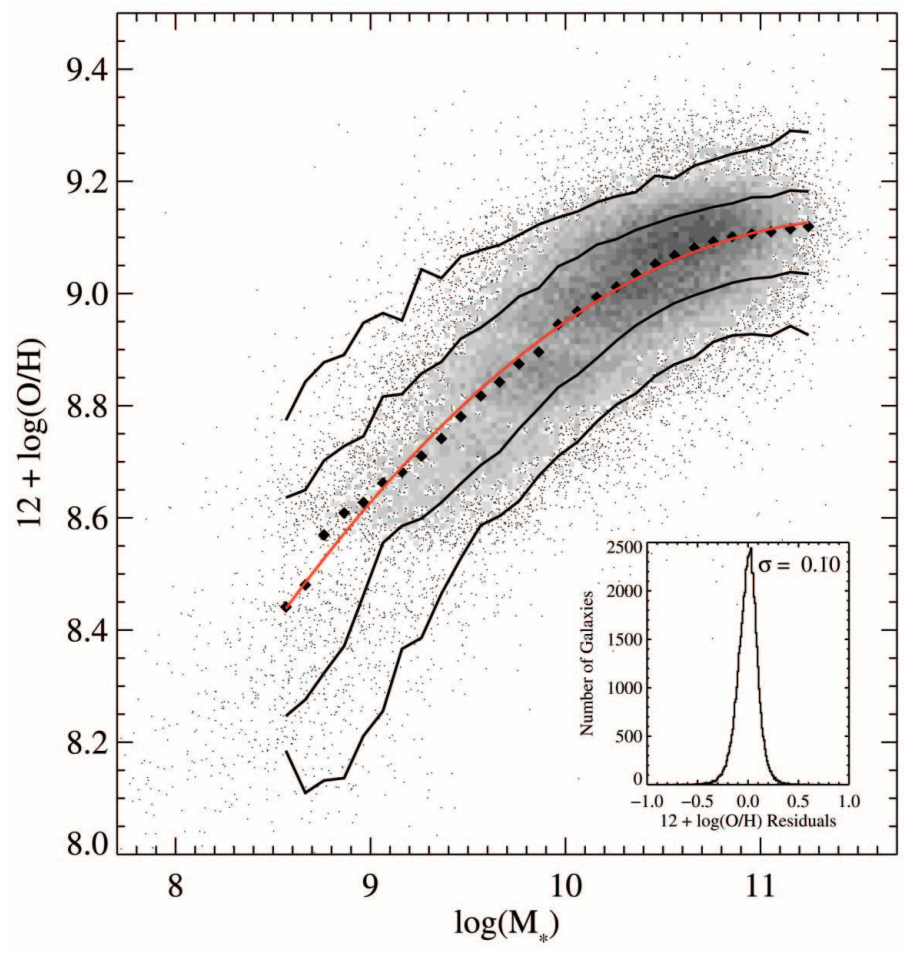
\includegraphics[width=\textwidth]{tremonti.png}
\caption{The observed mass--metallicity relation for star-forming
  galaxies in the Sloan Digital Sky Survey (Tremonti et
  al. 2004).}\label{fig:tremonti}
\end{figure}

\noindent{\bf (d; 2 parts of 3 points each)} The observed relation
between the oxygen abundance and the stellar mass of galaxies is shown
in Figure~\ref{fig:tremonti}. It is clear that there is a strong
correlation between the stellar mass and the oxygen abundance for
galaxies. \\

\noindent{\bf (d.1)} Why is oxygen a good element to measure to
investigate the relation between a galaxy's mass and its metal
abundance?\\

\noindent{\bf (d.2)} If you interpret this relation in the context of
the leaky-box chemical-evolution model, what are two options for
explaining the origin of this relation? Discuss these options in terms
of what we have learned this semester about dynamics and the structure
of galaxies.\\

\noindent{\bf Problem 2:} (18 points; 3 each) A popular method for
modifying gravity is replacing the Newtonian gravitational force with
a \emph{Yukawa force}. In such a model, particles feel a force
mediated through a massive, scalar particle instead of the standard
Newtonian $1/r^2$ force. Such an interaction gives rise to a Yukawa
potential $\Phi_y(r)$; specifically, an object with mass $M$ gives
rise to a potential
\begin{equation}\label{eq:yukawa_pot}
  \Phi_y(r) = -\frac{\alpha\,GM}{r}\,e^{-m_\phi\,r}\,,
\end{equation}
where $\alpha$ parameterizes the strength compared to that of standard
gravity and $m_\phi$ is the mass of the scalar mediator (in the
exponential we are using units in which $\hbar = c = 1$). Let's
investigate these types of models and how well they are constrained!\\

\noindent{\bf{ (a)}} Re-write Equation~\eqref{eq:yukawa_pot} as
\begin{equation}
  \Phi_y(r) = -\frac{\alpha\,GM}{r}\,e^{-r/\lambda}\,,
\end{equation}
by converting $m_\phi$ to a length scale using $\hbar$ and $c$. In
particular, what $m_\phi$ does $10^{12}\,\mathrm{km}$ correspond to
(express $m_\phi$ in eV)?\\

\noindent{\bf{ (b)}} Does Newton's first shell theorem hold if the
gravitational force is of the Yukawa type rather than Newtonian?
Explain why or why not.\\

\noindent{\bf{ (c)}} Explore what orbits look like in a Yukawa
potential. You can do this by considering the effective potential and
looking at orbits that are either near to or far from circular. Some
cases to consider: $r \ll \lambda$, $r = \lambda$, $r = 2\lambda$, and
$r \gg \lambda$.\\

\noindent{\bf{ (d)}} Circular orbits in a spherical potential are
stable if orbits close to a circular orbit oscillate around the
circular orbit. In the epicycle formalism, what constraint does this
set on the epicycle frequency? (Hint: consider the relation between the
epicycle frequency and the curvature of the effective
potential.) Using this constraint, find the maximum $r/\lambda$ where
stable circular orbits exist in a Yukawa potential. Given that galaxy
clusters appear to be gravitationally bound, what kind of constraint
on $\lambda$ can you derive from this (express in km and also in terms
of $m_\phi$ in eV)?\\

\noindent{\bf{ (e)}} Yukawa-type forces can be constrained by using
the fact that the orbit of the Moon around the Earth or the orbits of
planets around the Sun close to within measurement
uncertainties---after accounting for small deviations stemming from
the general theory of relativity and the Earth/Sun's quadrupole
moment. Compute, analytically, the precession $2\pi-\Delta \psi$ of
the apocenter in a Yukawa potential for a near-circular orbit in terms
of $\alpha$, $\lambda$, and the radius $r$ of the circular orbit. From
observations of Mercury and Mars' orbits, we can determine that
$|2\pi-\Delta \psi| \lesssim 100$ nanoradians. For $\alpha \approx
1$---i.e., gravity is fully Yukawa---what constraint does this put on
$\lambda$ (express in km) and, thus, $m_\phi$ (express in eV)? For
reference, the LIGO constraints on $m_\phi$ are $m_\phi \lesssim
10^{-22}\,\mathrm{eV}$ (these come from the fact that a massive
graviton leads to frequency-dependent travel-times for gravitational
waves, constrained by the observed binary-black-hole mergers, and to a
slower propagation speed of gravitational waves compared to the speed
of light, constrained by the near-coincidence of the
gravitational-wave and electromagnetic emission in the binary
neutron-star merger GW170817).\\

\noindent{\bf{ (f)}} Rather than being a full-on replacement of
Newtonian gravity, Yukawa-type forces may also be present \emph{in
  addition} to gravity. For example, in some dark matter models, dark
matter feels an additional Yukawa force (with strength $\alpha$
relative to Newtonian gravity) in addition to standard gravity, while
ordinary matter does not feel the additional force.  At scales $r \gg
m_\phi^{-1}$, such a force acts as an additional gravitational force
between dark-matter particles and can therefore be modeled as a simple
change in the gravitational constant for such particles: $\tilde{G} =
G\,(1+\alpha)$. Discuss how this additional interaction affects the
following types of observations if we interpret them assuming that
gravity is the only force (that is, how does the inferred mass relate
to the true mass):

\begin{itemize}
\item The matter distribution in disk galaxies inferred from their
  rotation curves.
\item The mass of the Milky Way inferred from the velocities of halo globular clusters.
\item The mass of the Milky Way inferred by assuming that a distant satellite (e.g., Leo I) moves at the escape velocity.
\item The mass of the Local Group determined using the timing
  argument.
\end{itemize}

%\noindent{\bf{ (g)}} For standard Newtonian gravity, we know that the
%relation between the gravitational potential and the density is given
%by the Poisson equation. Derive the relation between $\Phi_y$ and
%$\rho$ if gravity follows the Yukawa potential rather than the
%standard Newtonian $\Phi_N \propto -GM/r$ law.\\

\noindent{\bf Problem 3:} (7 points) Conservation laws and numerical
integration. Consider an $N$-body system under unsoftened, Newtonian
gravity. Write a simple $N$-body integrator that uses i) direct
summation to obtain the forces and ii) both the leapfrog and
fourth-order Runge-Kutta method for orbit integration of the $N$
bodies. Compare the conservation of total angular momentum $\sum_i
m_i\,\vec{x}_i\times\vec{v}_i$ when using a constant (small) time step
between the leapfrog and Runge-Kutta integrators. (Note: you are free
to choose $N$, but do not make it \emph{too} small). You should evolve
your system for about 100 dynamical times. Explain what you see in
terms of the theory behind the different integrators.

\newpage

\section*{Selected questions from the General Qualifying Exam:}

After having this course, you should be able to answer the following
questions from the General Qualifying Exam:

\begin{itemize}
\item What is the total mass (in both dark matter and in stars) of the
  Milky Way galaxy? How does this compare to M31 and to the LMC? How
  is this mass determined?
\item Define and describe globular clusters. Where are they located?
  What are their typical ages, and how is this determined?
\item Describe a dynamical method used in the determination of the
  mass of a galaxy cluster. (Note: full question asks for three
  methods, not solely dynamical).
\item Draw the spectral energy distribution (SED) of a galaxy formed
  by a single burst of star formation at the ages of 10 Myrs, 2 Gyrs,
  and 10 Gyr. Please highlight the change over time in the 4000
  Angstrom break.
\item What are galaxy clusters? What are their basic properties (e.g.,
  mass, size). [We'll skip this part: List and explain three ways they
    can be detected.]
\item Describe the orbits of stars in a galactic disk and in a
  galactic spheroid.
\item Galactic stars are described as a collisionless system. Why?
\item The stars in the solar neighborhood, roughly the 300 pc around
  us, have a range of ages, metallicities, and orbital properties. How
  are those properties related?
\item What is dynamical friction? Explain how this operates in the
  merger of a small galaxy into a large one.
\item Sketch the rotation curve for a typical spiral galaxy. Show that
  a flat rotation curve implies the existence of a dark matter halo
  with a density profile that drops off as $1/r^2$.
\item Characterize the stellar populations in the following regions:
  i) the Galactic bulge, ii) the Galactic disk, outside of star
  clusters, iii) open star clusters, iv) globular clusters, v) a
  typical elliptical galaxy.
\item What is the G-dwarf problem in the solar neighborhood?
\item Describe the general characteristics of spiral structure in
  galaxies.
\end{itemize}

\end{document}
